\documentclass{beamer}
\usetheme{Madrid} % Clean theme
\usepackage{listings}
\usepackage{xcolor}
\usepackage{graphicx}

\usepackage{gvv}

% Code listing style
\lstset{
  basicstyle=\ttfamily\footnotesize,
  keywordstyle=\color{blue},
  stringstyle=\color{orange},
  commentstyle=\color{green!60!black},
  breaklines=true,
  frame=single,
  showstringspaces=false
}

\title{MatGeo Assignment - Problem 1.9.13}
\author{EE25BTECH11024}
\institute{IIT Hyderabad}

\begin{document}

% Title slide
\begin{frame}
  \titlepage
\end{frame}

% Problem statement
\begin{frame}{Problem Statement}
A man goes 5 meters due west and then 12 meters due north. How far is he
from the starting point?
\end{frame}

% Solution using Rank Criterion (Slide 1)
\begin{frame}{Solution:}
\noindent
Let's assume that the man starts from the origin. He moves 5 m west to point A.
\begin{align}
    \vec{A} = 5\myvec{-1 \\ 0}
\end{align}

He then moves 12m north from B.
\begin{align}
    \vec{B} = 5\myvec{-1 \\ 0} + 12\myvec{0 \\ 1} = \myvec{-5 \\ 12}
\end{align}

Therefore the corrdinates are

\begin{center}
    \begin{tabular}{|c|c|c|}
    \hline
    \textbf{Symbol} & \textbf{Value} & \textbf{Description}  \\
    \hline
    \textbf{\vec{0}}      & \myvec{0 \\ 0}         & Origin        \\
    \hline
    \textbf{\vec{A}}      & \myvec{-5 \\ 0}        & First Point   \\
    \hline
    \textbf{\vec{B}}      & \myvec{-5 \\ 12}      &Second Point    \\
    \hline
    \end{tabular}
\end{center}

\end{frame}

% Solution using Rank Criterion (Slide 2)
\begin{frame}{Solution: }
\noindent
We need to find the distance between the starting point O and the final point B.

\begin{align}
    \vec{O} - \vec{B} = \myvec{0 \\ 0} - \myvec{-5 \\ 12} = \myvec{5 \\ -12}
\end{align}

\begin{align}
    (\vec{0} - \vec{B})^\top(\vec{0} - \vec{B}) = 169 = \|0 - B\|^2
\end{align}

Thus the desired distance is
\begin{align}
    d = \|\vec{O} - \vec{B}\| = \sqrt{169} = 13
\end{align}

The distance between the man and the starting point = 13
See Figure~\ref{fig:pathofman}.

\end{frame}

\begin{frame}{Resulting Graph}
\centering
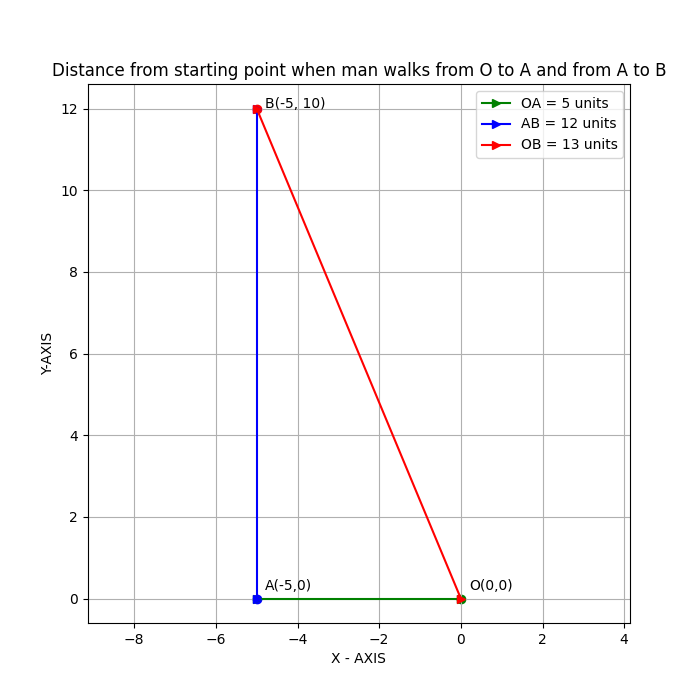
\includegraphics[width=0.6\linewidth]{figs/fig2.png}
\caption{}
\label{fig:pathofman}
\end{frame}

% Python code 1
\begin{frame}[fragile]{Python Code: plot.py (Native)}
\begin{lstlisting}[language=Python]
import numpy as np
import matplotlib.pyplot as plt

A = np.array([-5, 0])
B = np.array([-5, 12])
O = np.array([0, 0])

plt.figure(figsize = (7,7))
plt.plot([O[0], A[0]], [O[1],A[1]], 'g->', label = 'OA = 5 units')
plt.plot([A[0], B[0]], [A[1],B[1]], 'b->', label = 'AB = 12 units')
plt.plot([B[0], O[0]], [B[1],O[1]], 'r->', label = 'OB = 13 units')

plt.scatter(*O, color = "green")
plt.scatter(*A, color = "blue")
plt.scatter(*B, color = "red")

plt.text(O[0]+0.2, O[1]+0.2, "O(0,0)")
plt.text(A[0]+0.2, A[1]+0.2, "A(-5,0)")
plt.text(B[0]+0.2, B[1], "B(-5, 10)")
\end{lstlisting}
\end{frame}


\begin{frame}[fragile]{Python Code (Native Implementation – plot.py)}
\begin{lstlisting}[language=Python]
plt.xlabel("X - AXIS")
plt.ylabel("Y-AXIS")
plt.title("Distance from starting point when man walks from O to A and from A to B")
plt.legend()
plt.grid(True)
plt.axis("equal")
plt.savefig("fig2.png")
plt.show()
\end{lstlisting}
\end{frame}

\begin{frame}[fragile]{C Code (Shared Library – finddistance.c)}
\begin{lstlisting}[language=C]
#include <stdio.h>
#include <math.h>

double find_distance(double x1, double y1, double x2, double y2){
    double d = sqrt(pow(x2-x1, 2) + pow(y2-y1, 2));
    return d;
}
\end{lstlisting}
\end{frame}

% Python code 2
\begin{frame}[fragile]{Python Code: call.py (C + Python)}
\begin{lstlisting}[language=Python]
import ctypes #for interacting with c code (datatypes such as .so)
import numpy as np
import matplotlib.pyplot as plt

so = ctypes.CDLL("./find_distance.so") #loads my shared c library so that python can use it

so.find_distance.argtypes = [ctypes.c_double, ctypes.c_double, ctypes.c_double, ctypes.c_double]
so.find_distance.restype = ctypes.c_double

O = np.array([0,0])
A = np.array([-5,0])
B = np.array([-5,12])

d_OA = so.find_distance(O[0], O[1], A[0], A[1])
d_AB = so.find_distance(A[0], A[1], B[0], B[1])
d_OB = so.find_distance(O[0], O[1], B[0], B[1])
\end{lstlisting}
\end{frame}

\begin{frame}[fragile]{Python Code (C Integrated – call.py)
}
\begin{lstlisting}[language=Python]
plt.figure(figsize = (7,7))
plt.plot([O[0], A[0]], [O[1], A[1]], 'g-', label = f"OA = {d_OA:.0f} units")
plt.plot([A[0], B[0]], [A[1], B[1]], 'b-', label = f"AB = {d_AB:.0f} units")
plt.plot([O[0], B[0]], [O[1], B[1]], 'r-', label = f"OB = {d_OB:.0f} units")

plt.scatter(*O, color = 'green')
plt.scatter(*A, color = 'blue')
plt.scatter(*B, color = 'red')

plt.text(O[0]+0.2, O[1]+0.2, "O(0,0)")
plt.text(A[0]+0.2, A[1]+0.2, "A(-5,0)")
plt.text(B[0]+0.2, B[1], "B(-5, 10)")
\end{lstlisting}
\end{frame}

\begin{frame}[fragile]{Python Code (C Integrated – call.py)
}
\begin{lstlisting}[language=Python]
plt.xlabel("X-AXIS")
plt.ylabel("Y-AXIS")
plt.title("Distance from starting point when man walks from O to A and from A to B")
plt.legend()
plt.axis('equal')
plt.grid(True)
plt.savefig("fig2'.png")
plt.show()
\end{lstlisting}
\end{frame}



\end{document}

